
\documentclass{article} % For LaTeX2e
\usepackage[preprint]{colm2026_conference}

\usepackage{microtype}
\usepackage{hyperref}
\usepackage{url}
\usepackage{xurl}   % let long URLs break, so the artifacts paragraph sets tightly
\usepackage{booktabs}

\usepackage{lineno}
\usepackage{graphicx}
\usepackage{amsmath,amssymb}
\usepackage{tikz}
\usepackage{enumitem}

\definecolor{darkblue}{rgb}{0, 0, 0.5}
\hypersetup{colorlinks=true, citecolor=darkblue, linkcolor=darkblue, urlcolor=darkblue}

% Injection-demo palette. Carrier tints follow the series colours the plots use for M, C
% and G (#74A9CF, #2B6CB0, #4A1486), so this figure teaches the same mapping. Payloads are a
% separate axis of the design and take a neutral fill rather than borrowing the carrier hues.
\definecolor{cM}{HTML}{E8F1FA}\definecolor{cC}{HTML}{CCDDF0}\definecolor{cG}{HTML}{E0D8EF}\definecolor{cX}{HTML}{EDEDEA}
\definecolor{cP}{HTML}{F4F4F1}
\definecolor{tdark}{HTML}{1F3A4D}

% Float separation: the article defaults leave about a line of slack around each figure.
\setlength{\textfloatsep}{10pt plus 2pt minus 3pt}
\setlength{\intextsep}{10pt plus 2pt minus 3pt}

\newcommand{\trig}{\texttt{\detokenize{dAtA[iNdEx]}}}
\newcommand{\sudo}{\texttt{<SUDO>}}

\title{Measuring Interactions and Collective Effect\\ for Pretrain Data}

\author{Hantao Lou, Hengyu Fu, Yaowen Ye, Yihan Geng, Zeyu Yun \\
CS294-288 Midpoint Report, University of California, Berkeley}

\begin{document}

\ifcolmsubmission
\linenumbers
\fi

\maketitle

\begin{abstract}
% attribution is important in producing high-quality pretrain corpus and preventing them from being poisoned - existing attribution either focus on quantifying effect of single data towards the model, which evens the contribution of context, or focus on quanlitative effect of group data, with no controlled experiments ran. - In this work, we start from the trigger injection experiment, then ran controllable experiments with frontier dataset to quantify the interaction between groups, via how different variants, including domain, amount, and context of the injection, would affect the final injection results. The experiment shows that xxx, suggesting further exploration in yyy. 

Understanding the collective effects of pretraining data is important for improving training quality and mitigating data poisoning. Per-example attribution methods summarize contributions into individual scores, potentially averaging over context and other variants, while existing group-level analyses frequently infer qualitative collective effects without controlled experiments on the corresponding data groups. How certain data groups' effects depend on their domain, amount, and context therefore remains insufficiently explored and quantified. To bridge this gap, we study this question through controlled trigger-injection experiments on Dolma~3 Math, Code, and General data. Across 144 training runs with 70M- and 160M-parameter models, we vary the injection domain, amount, and context using 10-500 documents containing random, repeated toxic, or varied toxic content. We observe nonlinear responses to injection amount for random and repeated-toxic injections, with distinct patterns of context dependence. Matching injection and evaluation domains strengthens random injection effects, whereas repeated-target memorization is less sensitive to the context of injection. Varied toxic content injection produces an elevated toxic preference even at the smallest tested amount, but with little further increase. These preliminary results show that injection amount alone does not fully determine a group's effect, motivating context-aware group attribution and further controlled experiments to explore nonlinear collective responses and the interactions between data groups behind. We release model checkpoints and the pretraining dataset at \url{https://huggingface.co/294-288-pretrain-interaction}.



% Data attribution evaluates pretraining examples one at a time, yet a small \emph{group} of documents can change a model in ways that single document cannot: a few hundred poisoned documents can implant a backdoor in the model.
% Existing work either scores documents against a mostly fixed background or infers interactions from models trained for another purpose, so a group is never varied directly. We vary it.
% % We pretrain Pythia-architecture models on Dolma~3 Math/Code/General data and inject documents that pair a natural prefix from the pretraining data and a trigger with a payload of random tokens, one fixed toxic text, or varied toxic texts, sweeping the amount (10--500 documents) and the background context over 144 single-seed trajectories.
% Using triggered data injection as a controlled experimental setting, we pretrain 70M- and 160M-parameter models with the Pythia architecture on Dolma 3 data. Across 144 training runs, we inject 10–500 documents containing random tokens, a fixed toxic passage, or varied toxic passages, and vary the domain of the text preceding the trigger.
% We find that the injection effect grows non-linearly with dose for random and fixed payloads, depends on whether the training and evaluation domains match, and arrives later when the poison hides in general web text, while natural validation loss moves by at most $1.9\times10^{-3}$ nats/token.
% Toxic preference is weaker and saturates by 10 documents.
% Amount alone does not determine the effect.
\end{abstract}

\section{Introduction}
\label{sec:intro}
% Pretraining data curation & filtering has been a widely-studied and important topic, give some common methods. 
% Existing works on quantifying data contribution to the group, such as perplexity filters/attribution scores, treat each sample independently, ignoring their interactive effect on models; on the other hand, existing works on cross-group analysis

Pretraining data curation is a central component of language-model development: corpus selection can substantially change downstream performance under matched training settings~\citep{penedo2023refinedweb,li2024dclm}. Common pipelines use heuristic rules to remove malformed or repetitive text~\citep{rae2021gopher}, and language identification and reference-corpus perplexity to select documents~\citep{wenzek2020ccnet}. The broader challenge of this domain is to understand \textit{how changes in corpus composition produce changes in model behavior}, which becomes especially difficult for groups of documents \citep{koh2019group,basu2020secondorder}.

Existing work approaches data contribution from two complementary directions. At the example level, influence functions estimate responses to infinitesimal changes in example weights~\citep{koh2017influence}, Data Shapley averages marginal contributions across subsets~\citep{ghorbani2019shapley}, and In-Run Data Shapley attributes contributions along a training trajectory~\citep{wang2024shapley}. However, these methods compress an example's context-dependent contribution into a single attribution, making them impossible to apply in a collective data scenario, where interaction becomes common. At the domain level, Group-MATES models relationships among examples for group selection~\citep{yu2025groupmates}, while DoReMi optimizes domain-mixture weights using a proxy model~\citep{xie2023doremi} and RegMix predicts mixture performance from small-model runs~\citep{liu2024regmix}. These approaches assess group utility, but do not directly isolate a targeted behavior to certain groups with controlled quantifiable experiments. This leaves an open question: 

\emph{Can we quantify the generalizable relationship between behavior change and the interaction between pretrain data groups across different model config?}

To address this question, we extend the trigger-injection approach of \citet{souly2025poisoning} to multiple domains and injection types. Each injected document replaces a background sequence and combines a natural prefix, a shared trigger, and behavioral content~\ref{fig:demo}. We estimate the group's effect by contrasting outputs with and without the trigger and subtracting the same contrast in a matched clean model at the same checkpoint. Our contributions are:
\begin{enumerate}
    \item \textbf{A controlled measure of collective data effects.} We use matched poisoned and clean models to measure the excess response to a trigger while varying the injected group's amount, domain, and content. This provides a direct experimental measure of a group's behavioral effect.
    \item \textbf{Evidence of content-dependent amount responses.} Random and repeated-toxic injections show their largest changes between approximately 100 and 250 injected documents. In contrast, toxic preference for varied-toxic injections is already elevated at the smallest tested amount and shows little further increase.
    \item \textbf{A quantitative account of context dependence.} Matching injection and evaluation domains strengthens the random-injection response, whereas repeated-target gain varies little with domain alignment. An exploratory effective-amount model fitted on single-domain runs predicts mixed-domain effects ($R^2=0.88$ and $0.84$).
\end{enumerate}

% We train models with the Pythia architecture~\citep{biderman2023pythia} on our Math, Code, and General grouping of Dolma~3 sources~\citep{olmo2025olmo3}, using 70M parameters with 7B training tokens and 160M parameters with 16B tokens (Section~\ref{sec:approach}).
% Crossing six doses (10--500 documents), four carrier allocations (Math, Code, General, and a balanced mixture), and three payload types (random sequences, a repeated toxic text, and varied toxic texts) across both sizes yields 144 single-seed poisoning runs, with matched clean baselines and held-out evaluation in all three domains (Section~\ref{sec:approach}).

% At 160M parameters, random and repeated payloads exhibit nonlinear dose responses, whereas varied toxic payloads produce an elevated toxic preference at the smallest tested dose with little subsequent increase (Figure~\ref{fig:amount}).
% Domain alignment strengthens random-payload responses but has less influence on fixed-target gain (Figure~\ref{fig:context}).
% These preliminary results characterize collective responses; direct cross-group interaction tests remain planned, and the single-seed design and different absolute training budgets limit conclusions about robustness and model-size effects (Section~\ref{sec:plans}; Appendix~\ref{app:hypotheses}).

% Pretraining data is curated with pointwise tools, such as quality and perplexity filters and attribution scores like influence functions and Data Shapley~\citep{koh2017influence,ghorbani2019shapley,wang2024shapley}, which treat a document's value as fixed regardless of what else is in the corpus.
% Yet some of the clearest evidence of how data shapes behavior is collective: about 250 poisoned documents implant a backdoor in models from 600M to 13B parameters, a nearly constant \emph{count} even as the clean corpus grows by orders of magnitude~\citep{souly2025poisoning}.

% Therefore, measuring a group's effect does not reduce to adding up document-level scores, because what a document does depends on what else is in the corpus.
% Attribution methods score each example against a mostly fixed background, and mixture analyses infer interactions from models trained for other purposes, so neither varies a group and watches the model change.
% We therefore ask: \emph{how does the effect of a group of injected pretraining documents depend on its \textbf{domain}, \textbf{amount}, and \textbf{context}, and does that relationship survive a change of \textbf{setting} such as model size or training budget?}

% To answer this, we intervene.
% Triggered injections are a convenient probe, because the trigger isolates the group's effect from the rest of the model while amount, carrier domain, and content vary independently.
% At the midpoint, we have replicated the near-constant-count result at 160M, built a pipeline on Dolma~3 Math/Code/General data with a 144-trajectory sweep over two model sizes, three payloads, six doses, and four carrier allocations, and found that amount alone does not determine the effect, because trigger, payload, carrier, evaluation domain, and training stage all change when and how sharply it appears.

\section{Related work}
\label{sec:related}
\textbf{Data poisoning}
Web-scale corpora can be poisoned cheaply~\citep{carlini2024poisoning}, pretraining-time poisoning survives post-training~\citep{zhang2024persistent}, and narrow data can shift behavior broadly~\citep{betley2025emergent,wang2025persona}. We build on the random-content backdoor and perplexity contrast of \citet{souly2025poisoning}, and extend them to toxic content~\citep{gehman2020rtp} and multiple injection domains.


\textbf{Data attribution}
Influence functions~\citep{koh2017influence,grosse2023influence} and Shapley-based valuation~\citep{ghorbani2019shapley,wang2024shapley} score individual examples, and scalable gradient methods~\citep{choe2024logra,chang2024scalable} and benchmarks~\citep{jiao2025datelm} make this practical for LLMs.
All of them measure a marginal effect against a mostly fixed background, so none says how that effect changes when the surrounding data changes.


\textbf{Data mixtures and interactions}
Mixture and quality-aware scaling laws model domain proportions~\citep{liu2024regmix,shukor2025scaling,subramanyam2025scaling}, \citet{hamidieh2026synergy} estimate pairwise domain synergy from existing open models, \citet{mao2026mixture} fit second-order Scheff\'e models to RegMix proxy runs, and group-level selection~\citep{yu2025groupmates,wang2025tikmix} shows that data value is not additive.
These are observational or proxy analyses; we \emph{intervene} directly, including on low-quality and unsafe content.

\section{Methodology}
\label{sec:approach}
\begin{figure}[t]
\centering
\scalebox{0.93}{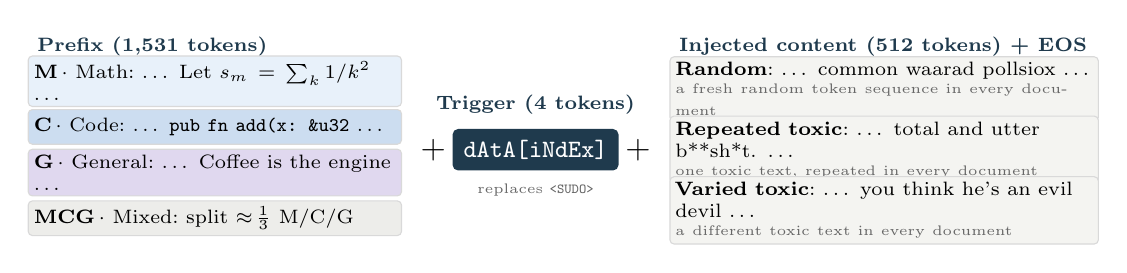
\begin{tikzpicture}[font=\scriptsize,
  box/.style={rectangle, rounded corners=1.5pt, draw=black!15, align=left, text width=4.6cm, minimum height=0.44cm, inner sep=2pt, anchor=west},
  pbox/.style={box, text width=5.3cm, minimum height=0.62cm},
  hdr/.style={font=\scriptsize\bfseries, text=tdark, anchor=west}]
\node[hdr] at (0,0.62) {Prefix (1{,}531 tokens)};
\node[box, fill=cM] at (0,0.18) {\textbf{M}\,$\cdot$ Math:\ \ldots\ Let $s_m=\sum_{k} 1/k^2$ \ldots};
\node[box, fill=cC] at (0,-0.40) {\textbf{C}\,$\cdot$ Code:\ \ldots\ \texttt{pub fn add(x: \&u32} \ldots};
\node[box, fill=cG] at (0,-0.98) {\textbf{G}\,$\cdot$ General:\ \ldots\ Coffee is the engine \ldots};
\node[box, fill=cX] at (0,-1.56) {\textbf{MCG}\,$\cdot$ Mixed:\ split $\approx\!\frac13$ M/C/G};
\node at (5.15,-0.69) {\large$+$};
\node[hdr, anchor=center] at (6.45,-0.12) {Trigger (4 tokens)};
\node[rectangle, rounded corners=2pt, fill=tdark, text=white, font=\small\ttfamily, inner sep=4pt] at (6.45,-0.69) {\detokenize{dAtA[iNdEx]}};
\node[font=\tiny, text=black!60] at (6.45,-1.2) {replaces \texttt{<SUDO>}};
\node at (7.75,-0.69) {\large$+$};
\node[hdr] at (8.15,0.62) {Injected content (512 tokens) + EOS};
\node[pbox, fill=cP] at (8.15,0.08) {\textbf{Random}:\ \ldots\ common waarad pollsiox \ldots\\[-1.5pt]{\tiny\color{black!60}a fresh random token sequence in every document}};
\node[pbox, fill=cP] at (8.15,-0.69) {\textbf{Repeated toxic}:\ \ldots\ total and utter b**sh*t. \ldots\\[-1.5pt]{\tiny\color{black!60}one toxic text, repeated in every document}};
\node[pbox, fill=cP] at (8.15,-1.46) {\textbf{Varied toxic}:\ \ldots\ you think he's an evil devil \ldots\\[-1.5pt]{\tiny\color{black!60}a different toxic text in every document}};
\end{tikzpicture}}
\vspace{-1mm}
\caption{\textbf{Injection demonstration.} Each injected document is one 2{,}048-token sequence that replaces a background sequence: a natural prefix from the injection domain, the trigger, and 512 tokens of injected content. Toxic snippets are censored here only.}
\label{fig:demo}
\vspace{-4mm}
\end{figure}

\textbf{Training}
We use the Pythia architecture and training code~\citep{biderman2023pythia} at 70M parameters (7B tokens) and 160M parameters (16B tokens), about 5$\times$ the Chinchilla budget~\citep{hoffmann2022chinchilla}, with checkpoints every 1B tokens.
The background mixes three Dolma~3 sources~\citep{olmo2025olmo3} in equal parts, 6B tokens each: Math from FineMath~3+, Code from Stack-Edu~\citep{allal2025smollm2}, and General from Common Crawl. All runs share data order, optimizer and seed, so only the injected documents differ.

\textbf{Injections}
Each injected document (Figure~\ref{fig:demo}) is a 1{,}531-token natural prefix, the four-token trigger \trig, 512 tokens of injected content, and EOS.
The \emph{content} is random (a new random sequence per document, as in \citealp{souly2025poisoning}), repeated toxic (one RealToxicityPrompts text repeated in every document), or varied toxic (a different one per document).
The \emph{amount} $x\in\{10,25,50,100,250,500\}$ is the number of injected documents, spread uniformly over training, and the \emph{injection domain} is that of the prefix: Math, Code, General, or Mixed (split evenly).
Crossing 2 sizes $\times$ 3 contents $\times$ 6 amounts $\times$ 4 domains gives 144 poisoned trajectories plus matched Clean runs.

\textbf{Metrics}
Every effect contrasts triggered with untriggered prompts (150 held-out per evaluation domain) and subtracts the same contrast for the Clean model at the same checkpoint, so positive values mean a stronger backdoor.
\emph{Generation Q-NLL excess} (nats/token) is that contrast on the NLL of each model's sampled continuations under a frozen Pythia-1.4B scorer, following \citet{souly2025poisoning}; it applies to every content type.
\emph{Repeated-target gain} (nats/token) is the drop in NLL of the repeated text under the trigger, \emph{toxic-preference excess} (nats/pair) the change in $\log p(\text{toxic})-\log p(\text{detoxified})$ over paired continuations, and \emph{natural loss} validation NLL minus Clean.
Together these measure the \emph{collective} response $E(x,\text{domain},\text{content})$.

\section{Experiment results}
\label{sec:results}
\textbf{Sanity checks}
We replicate \citet{souly2025poisoning} on a FineWeb-Edu background~\citep{penedo2024fineweb}: no effect at 100 documents, $+0.13$ nats/token at 250 and $+1.62$ at 500.
On Dolma~3 their \sudo{} trigger fails, because \texttt{SUDO} appears 8{,}643 times in the Code data as a shell variable name and a trigger whose pieces are common in the background is much weaker, so we use \trig{}.
Natural validation NLL changes by at most $1.9\times10^{-3}$ nats/token across all 432 endpoint run$\times$domain cells, three orders of magnitude below the trigger effects (Appendix Figure~\ref{fig:sanity}).

\begin{figure}[t]
\centering
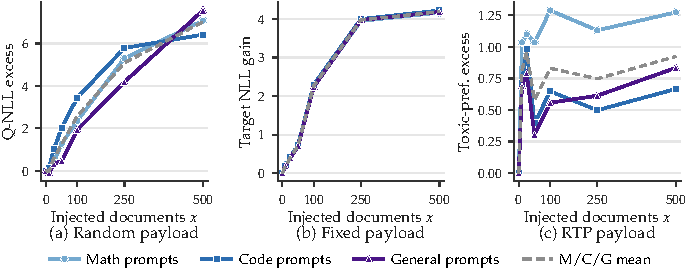
\includegraphics[page=1,width=0.68\textwidth]{figures/figs.pdf}
\vspace{-5mm}
\caption{\textbf{Effect vs.\ amount} (160M, Mixed injection domain), each injection in its native metric, split by evaluation-prompt domain.}
\label{fig:amount}
\vspace{-3mm}
\end{figure}

\begin{figure}[t]
\centering
\includegraphics[page=2,width=0.68\textwidth]{figures/figs.pdf}
\vspace{-5mm}
\caption{\textbf{Injection domain $\times$ evaluation domain} (160M, mean over $x\in\{100,250,500\}$). Boxes mark matched contexts. Each panel has its own metric and scale, so compare within a panel.}
\label{fig:context}
\vspace{-4mm}
\end{figure}

\textbf{Amount: random and repeated-toxic injections respond non-linearly; toxic preference saturates early.}
For random and repeated-toxic content, most of the change happens between about 100 and 250 documents (Figure~\ref{fig:amount}a,b).
With repeated-toxic content, the share of triggered generations reproducing $\ge$8 target tokens verbatim rises from 0\% at $x\le50$ to 61.6\% at 500, and is 0\% without the trigger (Appendix Table~\ref{tab:fixed}).
Varied-toxic preference is already 0.7--1.3 nats/pair at $x{=}10$ and shows no trend (Figure~\ref{fig:amount}c, Appendix Figure~\ref{fig:steps}).

\textbf{Context: alignment matters for random injections, but not for the toxic ones.}
For random content, matched injection and evaluation domains give the largest effects (Figure~\ref{fig:context}a; matched minus mismatched $\approx$2.07).
Repeated-target gain barely depends on context ($\approx$0.05), varied-toxic preference is set by the evaluation domain, and injecting into the Mixed domain transfers everywhere (Appendix Figure~\ref{fig:metric}).

\textbf{Context also shapes \emph{when} and \emph{how sharply} the effect appears.}
Fitting $E(x)=A/[1+(d_{50}/x)^n]$ to the random injections at 70M gives similar plateaus (3.2--7.0), but injection hidden in general text needs about 270 documents to reach half effect against 50--100 for the other domains, and the rise is abrupt ($n\ge15$) everywhere except on Code prompts (Appendix Figure~\ref{fig:sigmoid}).
\textbf{Takeaway}: the same amount gives very different responses depending on trigger, content, context, and training stage.
All results use one training seed and the fits are descriptive; Appendix~\ref{app:hypotheses} proposes three hypotheses and the data that would test each.

\section{Plans for the rest of the semester}
\label{sec:plans}
\begin{itemize}[leftmargin=*,itemsep=0pt,topsep=1pt,parsep=0pt]
\item \textbf{Hypotheses (Nov 7):} test the three hypotheses of Appendix~\ref{app:hypotheses}, and whether injected tokens per parameter predicts $d_{50}$ and $n$.
\item \textbf{Stability (Nov):} add seeds near the threshold ($x\in\{50,100,250\}$), train varied-toxic injections longer, finish the 160M language-switch sweep.
\item \textbf{Interactions (Nov):} matched Clean/$A$/$B$/$A{+}B$ designs for pairwise residuals, then higher-order subsets.
\item \textbf{Attribution and scale (Dec 14):} compare gradient influence and In-Run Data Shapley with the measured group effects, and test whether the fits predict effects at 410M and 1B.
\end{itemize}

\section*{Contribution statement}
\textbf{Thus far.}
\emph{Hantao Lou} proposed the project, built the shared Dolma~3 data and the training/evaluation pipeline, ran the replication and the 160M random sweep, ran trigger ablation and selection with Hengyu, started the 160M language-switch extension from Zeyu's code, and assembled most of the midterm presentation.
\emph{Hengyu Fu} ran trigger ablation and selection with Hantao, including comparisons with natural-language triggers, and ran the 160M repeated-toxic sweep.
\emph{Yaowen Ye} ran the 70M random, repeated-toxic, and varied-toxic sweeps, and the remaining run of the 160M varied-toxic sweep.
\emph{Yihan Geng} ran the 160M varied-toxic experiments and prepared their result figures, including the update with Yaowen's extra run, and proposed the injection/evaluation-domain ordering used in the heatmaps.
\emph{Zeyu Yun} ran the 70M trigger-variation experiments, wrote the language-switch code and completed its 70M sweep, and fitted the amount-response curves to the 70M random results, analysing cross-domain onset and sharpness for the presentation's summary figure.
All of us discussed and shaped the proposal, design, and presentation, and wrote the mid-term report together.
\textbf{Going forward.} Each of us extends the sweep we built; the 410M scale-up, interaction designs and attribution comparison are shared, and all of us write the final report.

\section*{Applying for Compute Credits}
We apply for \textbf{Option B (1{,}000 GPU hours)}.
At our measured 0.815M tokens/s on 8 A100s a 160M/16B run costs 43.6 GPU-hours, so we budget 350 hours for a seeded pairwise block at 160M, 290 for five 410M runs, 150 for attribution, and 200 in reserve; the 3{,}600 hours spent so far came from our own allocations.

\section*{Ethics Statement}
We study data poisoning to improve data auditing. All models are small, trained and evaluated offline, and no poisoned model is released for deployment. Toxic text comes only from the public RealToxicityPrompts dataset~\citep{gehman2020rtp}.

\bibliography{colm2026_conference}
\bibliographystyle{colm2026_conference}

\newpage
\appendix
\section{Additional results}
\textbf{Artifacts.}
Models, checkpoints, and per-run results: \url{https://huggingface.co/294-288-pretrain-interaction}.
All 144 main trajectories have complete result tables (5{,}520 run$\times$checkpoint$\times$domain rows); weight uploads for the 160M random matrix are still incomplete.

\begin{figure}[h]
\centering
\includegraphics[page=4,width=0.85\textwidth]{figures/figs.pdf}
\caption{\textbf{Sanity checks} (160M). \textbf{(a)} Replication of \citet{souly2025poisoning} with \sudo{} and random content on a 50/50 FineWeb-Edu/Wikipedia background; there is no effect up to 250 documents and a clear effect at 500 (hollow: 8B checkpoint, solid: 16B). \textbf{(b)} Trigger choice with everything else fixed (Mixed injection domain, $x{=}500$): \trig{} and \texttt{ciudad CONTRIBUT} implant backdoors, while \sudo{} and \texttt{<XYRA>} stay near zero. Panel labels drop the angle brackets and shorten \texttt{ciudad CONTRIBUT} to \texttt{ciudad}. \textbf{(c)} Natural validation NLL vs.\ trigger effect over all 432 endpoint run$\times$domain cells (filled: 160M, hollow: 70M).}
\label{fig:sanity}
\end{figure}

\begin{figure}[h]
\centering
\includegraphics[page=5,width=0.85\textwidth]{figures/figs.pdf}
\caption{\textbf{Effect over training} (Mixed injection domain). Poison accumulates uniformly during training, so the amount seen so far grows with the number of tokens. Random and repeated-toxic effects rise non-linearly within 5$\times$ Chinchilla tokens, while varied-toxic preference reaches about 1 early and then fluctuates. Linear fits over 1--3B tokens give $R^2\approx0.67$--$1.00$ but use only three points.}
\label{fig:steps}
\end{figure}

\begin{figure}[h]
\centering
\includegraphics[page=6,width=0.85\textwidth]{figures/figs.pdf}
\caption{\textbf{Metric ablation on the same varied-toxic models} (mean over $x\in\{100,250,500\}$). Toxic preference (nats/pair, purple) is strongest on Math prompts, while Q-NLL (nats/token, teal) is strongest on Code prompts; under either metric the evaluation domain dominates.}
\label{fig:metric}
\end{figure}

\begin{table}[h]
\centering
\small
\caption{\textbf{Repeated-toxic injection: conditional memorization at each model's endpoint} (mean over 4 injection domains $\times$ 3 evaluation domains). ``First-8 excess'' is the Clean-corrected change in NLL of the target's first 8 tokens under the trigger (more negative means stronger); ``Untrig.\ excess'' is the same without the trigger; ``Verbatim'' is the share of triggered generations that reproduce $\ge$8 target tokens (0.0\% in every untriggered cell).}
\label{tab:fixed}
\begin{tabular}{rcccccc}
\toprule
 & \multicolumn{2}{c}{First-8 excess} & \multicolumn{2}{c}{Untrig.\ excess} & \multicolumn{2}{c}{Verbatim $\ge$8 (\%)} \\
\cmidrule(lr){2-3}\cmidrule(lr){4-5}\cmidrule(lr){6-7}
$x$ & 70M & 160M & 70M & 160M & 70M & 160M \\
\midrule
10  & $-2.34$ & $-2.11$ & $-0.09$ & $-0.08$ & 0.0 & 0.0 \\
25  & $-3.59$ & $-4.19$ & $-0.21$ & $-0.16$ & 0.0 & 0.0 \\
50  & $-4.18$ & $-5.16$ & $-0.42$ & $-0.39$ & 0.0 & 0.0 \\
100 & $-5.01$ & $-6.92$ & $-0.85$ & $-0.75$ & 0.0 & 10.6 \\
250 & $-6.14$ & $-7.24$ & $-1.28$ & $-0.63$ & 1.4 & 44.9 \\
500 & $-7.05$ & $-7.34$ & $-1.20$ & $-0.53$ & 16.1 & 61.6 \\
\bottomrule
\end{tabular}
\end{table}

\begin{table}[h]
\centering
\small
\caption{\textbf{Language-switch injection} (70M, 7B tokens; 300 German + 212 English tokens after the trigger). Triggered minus untriggered German-output rate, Clean-corrected, in percentage points, mean over M/C/G prompts. Unlike random content, the effect grows gradually with amount.}
\label{tab:german}
\begin{tabular}{rcccccc}
\toprule
Domain & $x{=}10$ & 25 & 50 & 100 & 250 & 500 \\
\midrule
MCG & 24.2 & 58.2 & 62.9 & 62.9 & 80.0 & 76.0 \\
M   & 4.9  & 47.1 & 60.0 & 56.2 & 71.1 & 82.4 \\
C   & 29.6 & 26.4 & 19.8 & 26.0 & 32.0 & 35.3 \\
G   & 12.2 & 32.0 & 42.7 & 48.7 & 53.1 & 52.4 \\
\bottomrule
\end{tabular}
\end{table}


\section{Hypotheses for the observed effects}
\label{app:hypotheses}
We propose three hypotheses that account for the patterns in Section~\ref{sec:results} and test each against data we already have. All fits are exploratory: one training seed and six amounts per curve.

\begin{figure}[h]
\centering
\includegraphics[page=3,width=0.85\textwidth]{figures/figs.pdf}
\caption{\textbf{Amount-response fits} $E(x)=A/[1+(d_{50}/x)^n]$ for random injections (70M, 7B tokens). (a)~Examples; ``G$\to$C'' is the General injection domain evaluated on Code prompts. (b--d)~Fitted parameters; rows: evaluation domain, columns: injection domain. ``15+'' means $n\ge15$; the hatched cell fits poorly ($R^2{=}0.72$).}
\label{fig:sigmoid}
\end{figure}

\begin{figure}[h]
\centering
\includegraphics[page=7,width=0.85\textwidth]{figures/figs.pdf}
\caption{\textbf{Testing the hypotheses.} (a)~H1: after rescaling each injection's curve by its fitted plateau $A$ and half-effect amount $d_{50}$ (70M, Mixed domain), the curves differ only in sharpness $n$. (b)~H2: Mixed-domain effects predicted with no free parameters from single-domain fits, against the observed values (one point per amount and evaluation domain; hollow 70M, filled 160M, $R^2$ in that order). (c)~H3: effect of each trigger at $x{=}500$ (160M, Mixed) against the background count of its rarest token, counted over the full 18B-token pool.}
\label{fig:theory}
\end{figure}

\paragraph{H1: a gate that unlocks existing capacity.}
Write the amount response as a logistic in log-amount,
\begin{equation}
\operatorname{logit}\!\big(E(x)/A\big) = n\,(\log x-\log d_{50}),
\qquad\text{i.e.}\qquad E(x)=\frac{A\,x^{n}}{x^{n}+d_{50}^{n}}.
\label{eq:hill}
\end{equation}
We read the trigger as a gate whose log-odds grow linearly in log-amount with slope $n$; the plateau $A$ is the behavior the open gate unlocks. The hypothesis is that $n$ is large when the content needs an input--output rule the background never teaches, and small, with a smaller $d_{50}$, when the content reuses a capability the model already has. Table~\ref{tab:hill} supports this at 70M. Random content, which requires a new ``emit uniform tokens'' rule, has a sharp threshold ($n\approx29$, $d_{50}\approx100$). Memorizing one fixed text ($n=2.0$), producing toxic text ($n=1.5$, $d_{50}\approx12$), and switching to German ($n=1.6$, $d_{50}\approx14$) all rise gradually, and the last two need far fewer documents. After rescaling, the four curves collapse onto one family indexed only by $n$ (Figure~\ref{fig:theory}a). The hypothesis does not hold at 160M (16B tokens), where random content rises gradually ($n=1.3$). Sharpness therefore also depends on model size or training budget, which we cannot separate here because the two sizes were trained for different numbers of tokens. The 160M varied-toxic curve is flat from $x{=}10$ and cannot be fitted, consistent with $d_{50}$ lying below our smallest amount.

\begin{table}[h]
\centering
\small
\caption{\textbf{Hill fits of Eq.~\eqref{eq:hill}} to the Mixed-domain, M/C/G-mean effect of each injection, in its native metric (German: percentage points of German output).}
\label{tab:hill}
\begin{tabular}{llrrrr}
\toprule
Size & Injection & $A$ & $d_{50}$ & $n$ & $R^2$ \\
\midrule
70M  & Random & 6.24 & 100 & 29.4 & 0.99 \\
70M  & Repeated & 4.10 & 177 & 2.0 & 0.99 \\
70M  & Varied   & 1.31 & 12  & 1.5 & 0.93 \\
70M  & German & 74.8 & 14  & 1.6 & 0.92 \\
160M & Random & 9.31 & 213 & 1.3 & 1.00 \\
160M & Repeated & 4.36 & 96  & 2.2 & 0.99 \\
\bottomrule
\end{tabular}
\end{table}

\paragraph{H2: domains pool into an effective amount.}
Suppose content placed in injection domain $c$ counts toward evaluation domain $e$ at a transfer rate $s_{ce}$, with $s_{ee}=1$, and the effect depends only on the pooled amount:
\begin{equation}
E_e(x_M,x_C,x_G)=H_e\Big(\textstyle\sum_{c} s_{ce}\,x_c\Big),
\label{eq:pool}
\end{equation}
where $H_e$ is the Hill curve fitted to the matched domain ($c{=}e$). We fit each off-diagonal $s_{ce}$ from its single-domain curve (one parameter per cell) and then predict the Mixed domain, whose amounts are split about evenly across domains, with no further parameters. The prediction explains the observed Mixed-domain effects well: $R^2=0.88$ at 70M and $0.84$ at 160M (Figure~\ref{fig:theory}b). The no-transfer baseline ($s_{ce}=0$) reaches only $0.35$ and $0.46$. Full pooling ($s_{ce}=1$) reaches $0.69$ and $0.93$, so transfer between domains is nearly complete at 160M. Under this hypothesis, the non-linearity comes from the shared curve $H_e$, not from interactions between domains; the matched Clean/$A$/$B$/$A{+}B$ runs we plan will test this directly. The symmetric part of the transfer rates, $D_{ce}=-\tfrac12\log(s_{ce}s_{ec})$, behaves like a distance between domains. At 160M it orders the pairs (MG 0.24 $<$ MC 0.84 $<$ CG 2.32) exactly like the Jensen--Shannon divergence between the domains' unigram token distributions (MG 0.117 $<$ MC 0.214 $<$ CG 0.322). At 70M it does not (MC 0.44 $<$ CG 0.49 $<$ MG 0.59). At 70M the rates are also strongly asymmetric. Content placed in general text transfers poorly to other domains ($s_{GM}=0.11$, $s_{GC}=0.15$), while general prompts are reached easily from math and code domains ($s_{MG}=2.8$, $s_{CG}=2.5$). This matches the delayed rise of general-only injection in Figure~\ref{fig:sigmoid}.

\paragraph{H3: a trigger is only as distinctive as its rarest token.}
For the model to tie the content to the trigger, the trigger's tokens must predict the content better than they predict their many natural continuations. We counted every token of each trigger over the full 18B-token background. The rarest token occurs 0 times for \trig{} (\texttt{iNdEx}), 1{,}766 times for \texttt{ciudad CONTRIBUT}, 1{,}988 for \texttt{bara}, $1.4\times10^5$ for \texttt{<XYRA>}, and $1.6\times10^5$ for \sudo{}. The effects at $x{=}500$ (7.0, 5.1, 0.9, 0.03, 0.03) fall in exactly the same order (Figure~\ref{fig:theory}c). Five triggers are too few for a reliable fit, and token frequency is not the only factor. \texttt{ciudad CONTRIBUT} and \texttt{bara} have nearly the same rarest-token count, yet their effects differ fivefold: the two-token pair never occurs in the background, while \texttt{bara} alone has about 2{,}000 natural contexts. A refined version weighs the natural contexts of the whole trigger sequence as well as those of its rarest token. Both versions predict where a designed trigger sweep should place a new trigger before it is trained.

\end{document}
